\documentclass[12pt,a4paper]{article}
\usepackage[utf8]{inputenc}
\usepackage[spanish]{babel}
\usepackage{graphicx}
\usepackage{geometry}
\usepackage{amsmath}
\usepackage{booktabs}
\usepackage{listings}
\usepackage{xcolor,float, hyperref}
\geometry{margin=2cm}

% Configuración de listings para código Python
\lstset{
    language=Python,
    basicstyle=\ttfamily\small,
    keywordstyle=\color{blue},
    stringstyle=\color{red},
    commentstyle=\color{gray},
    frame=single,
    breaklines=true,
    showstringspaces=false
}

\title{Clasificación de Flores Iris con Regresión Lineal}
\author{Alejandro Flórez Lesmes \\ 
        Yeffersson Stiven Castro \\
        Universidad de Cundinamarca}
\date{\today}

\begin{document}

\maketitle

\section{Introducción}
El dataset de flores Iris es uno de los conjuntos de datos más famosos y utilizados en el campo del aprendizaje automático para problemas de clasificación. Generalmente, los modelos alcanzan precisiones muy altas, a menudo del 100\%, debido a la fuerte capacidad predictiva de las medidas del pétalo de las flores.

Sin embargo, un rendimiento perfecto en un entorno de laboratorio puede ser engañoso y no representa los desafíos de los problemas del mundo real, donde las clases a menudo se superponen. Por esta razón, este informe documenta un experimento donde se restringe el análisis a las características del \textbf{sépalo} (\textit{Sepal Length} y \textit{Sepal Width}), las cuales son conocidas por tener una menor capacidad de separación entre las especies \textit{Iris-versicolor} e \textit{Iris-virginica}.

El objetivo principal es doble: primero, comparar el rendimiento de un modelo de \textbf{Regresión Lineal} contra un modelo de \textbf{Regresión Logística} adaptado para clasificación; y segundo, analizar críticamente cómo la elección de características menos informativas crea un problema más realista y reduce la precisión del modelo, obligándonos a interpretar sus errores.

\section{Metodología}
El proceso de análisis se implementó en un script de Python utilizando librerías estándar del ecosistema de ciencia de datos. Los pasos metodológicos fueron los siguientes:

\subsection{Preparación de los Datos}
Se cargó el dataset \texttt{Iris.csv} utilizando la librería \texttt{pandas}. Las etiquetas categóricas de la columna \texttt{Species} ('Iris-setosa', 'Iris-versicolor', 'Iris-virginica') fueron transformadas a valores numéricos (0, 1, 2) mediante un \texttt{LabelEncoder} de \texttt{scikit-learn} para hacerlas compatibles con los modelos.

\subsection{Selección de Variables y División del Conjunto}
De acuerdo con el objetivo del estudio, se seleccionaron únicamente dos características para el entrenamiento:
\begin{itemize}
    \item \texttt{SepalLengthCm} (Largo del Sépalo)
    \item \texttt{SepalWidthCm} (Ancho del Sépalo)
\end{itemize}
Posteriormente, el conjunto de datos fue dividido en un 80\% para entrenamiento y un 20\% para pruebas, utilizando una semilla aleatoria (\texttt{random\_state=42}) para garantizar la reproducibilidad de los resultados.

\subsection{Entrenamiento de Modelos}
Se entrenaron dos modelos diferentes con los datos de entrenamiento:
\begin{enumerate}
    \item \textbf{Regresión Lineal:} Aunque es un modelo para regresión, se utilizó para predecir un valor continuo que luego fue redondeado y acotado para simular una clasificación. Se incluye como punto de referencia de un modelo no ideal.
    \item \textbf{Regresión Logística:} Es el modelo principal de estudio, diseñado específicamente para problemas de clasificación.
\end{enumerate}

\subsection{Evaluación}
La métrica principal para evaluar el rendimiento fue la \textbf{exactitud (accuracy)}, que mide la proporción de predicciones correctas. Los resultados obtenidos en la consola fueron los siguientes:

\begin{lstlisting}[caption={Salida de Precisión de los Modelos}, label=list:accuracy]
  Precision comparativa:
 - Regresion Lineal: 86.67%
 - Regresion Logistica: 90.00%
\end{lstlisting}

La Regresión Logística obtuvo un rendimiento superior, como era de esperar. Ambos modelos mostraron una precisión significativamente menor al 100\%, confirmando que las características del sépalo presentan un desafío de clasificación.

\newpage
\section{Resultados y Gráficos}
El análisis visual es fundamental para comprender por qué los modelos no alcanzan una precisión perfecta.

\subsection{Gráfico 1: Dispersión de Características del Sépalo}
Este gráfico (Figura \ref{fig:dispersion}) visualiza la distribución de las tres especies de Iris en el espacio definido por las medidas del sépalo.

\begin{figure}[H]
    \centering
    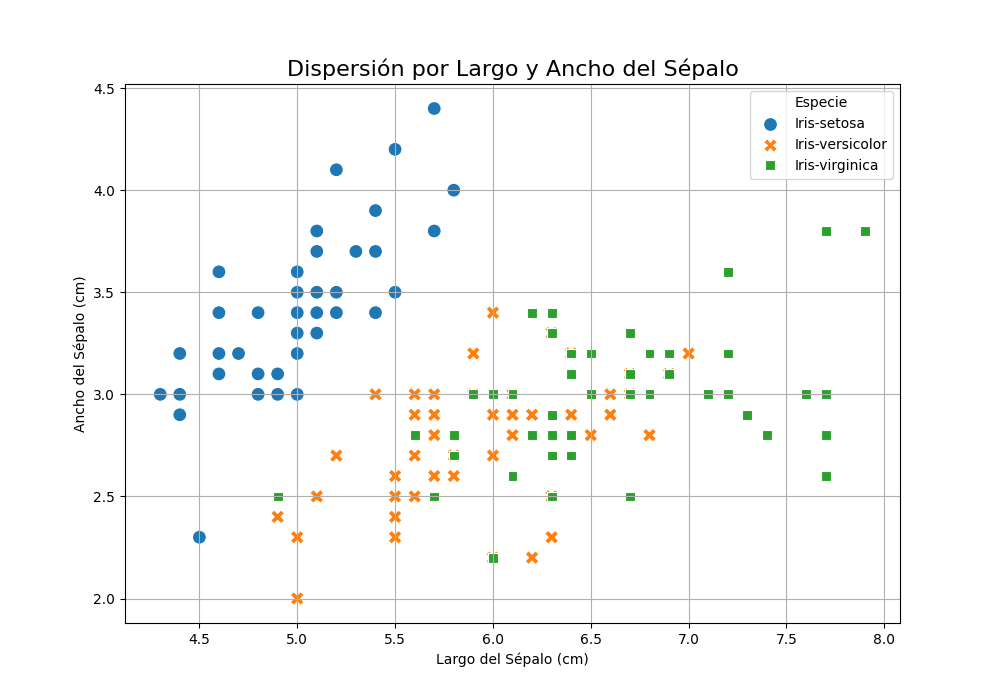
\includegraphics[width=0.8\textwidth]{Graficos/1_dispersion_sepalos.png}
    \caption{Distribución de las especies de Iris según las medidas del sépalo. Se observa un claro solapamiento entre Iris-versicolor e Iris-virginica.}
    \label{fig:dispersion}
\end{figure}

Como se puede apreciar, mientras que \textit{Iris-setosa} (en azul) forma un clúster claramente separable, los puntos correspondientes a \textit{Iris-versicolor} (naranja) e \textit{Iris-virginica} (verde) están considerablemente mezclados. Este solapamiento es la causa principal de los errores de clasificación.

\subsection{Gráfico 2: Matriz de Confusión del Modelo Lineal}
La matriz de confusión (Figura \ref{fig:confusion}) detalla los aciertos y errores del modelo de Regresión Lineal adaptado sobre el conjunto de prueba.

\begin{figure}[H]
    \centering
    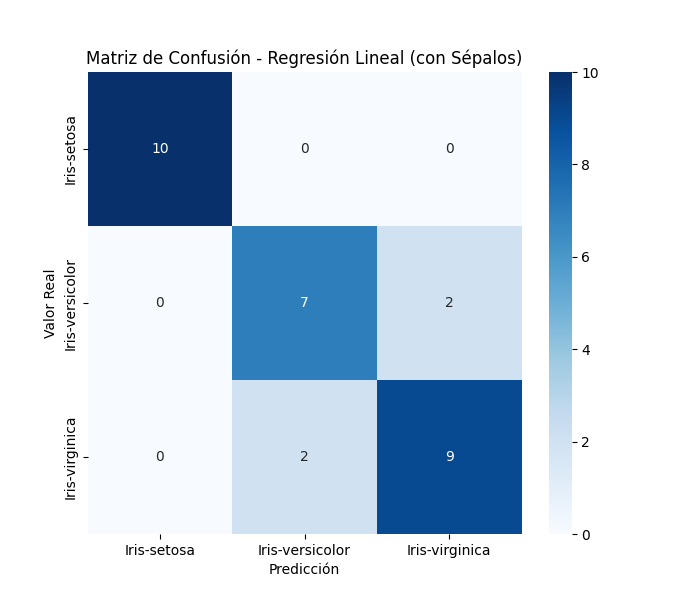
\includegraphics[width=0.6\textwidth]{Graficos/2_matriz_confusion.png}
    \caption{Matriz de confusión para el modelo de Regresión Lineal.}
    \label{fig:confusion}
\end{figure}

La diagonal principal muestra las predicciones correctas. Los valores fuera de la diagonal indican errores. En este caso, el modelo clasificó incorrectamente dos \textit{Iris-versicolor} como \textit{Iris-virginica}, lo cual es consistente con el solapamiento observado en la Figura \ref{fig:dispersion}.

\section{Discusión Crítica}
El experimento demuestra una lección fundamental en el aprendizaje automático: \textbf{la calidad de las características es a menudo más importante que la complejidad del modelo}. A pesar de utilizar algoritmos capaces, la precisión se vio limitada por la información inherente en los datos de entrada.

Al forzar a los modelos a usar solo las medidas del sépalo, simulamos un escenario común en problemas reales donde no existen características "perfectas" que separen las clases de manera trivial. La caída de la precisión del 100\% (obtenible con las características del pétalo) a un ~90\% refleja esta dificultad añadida.


\section{Conclusiones}
Del presente análisis se desprenden las siguientes conclusiones:
\begin{enumerate}
    \item La \textbf{Regresión Logística} es más adecuada para tareas de clasificación que la Regresión Lineal adaptada, obteniendo una mayor precisión en el problema planteado.
    \item La \textbf{selección de características} es un paso crítico que define el límite superior del rendimiento de un modelo. Las características del sépalo del dataset Iris no permiten una separación lineal perfecta entre todas las especies.
    \item El \textbf{análisis visual}es una herramienta indispensable para diagnosticar por qué un modelo comete errores y para entender la estructura intrínseca de los datos.
    \item Al limitar las características, se logró transformar un problema de libro de texto en un \textbf{escenario de clasificación más realista}, donde la superposición de clases es la norma.
\end{enumerate}

\textbf{Repositorio del Proyecto:} 
\url{https://github.com/StivenCastro138/Machine_Learning-Modelo2-.git}

\end{document}
